\documentclass{beamer}
%\usetheme{Antibes}
\usepackage{xcolor, colortbl}
\usepackage{algorithm}
\usepackage{algpseudocode}
\usepackage{textcomp}
\usepackage{listings}
\usepackage{hyperref}
\usepackage{alltt}
\usepackage{tikz}
\usepackage{framed}
\usepackage{marvosym}
\usepackage{wasysym}
\usepackage{marvosym}
\usepackage{crayola}
\usepackage{mathpartir}
\usepackage{tabularx}
\usepackage[belowskip=-15pt,aboveskip=0pt]{caption}
\usepackage[skins]{tcolorbox}
\usepackage{multicol}
\usetikzlibrary{positioning,shapes,arrows, arrows.meta, backgrounds, fit, shadows, automata}
\usetikzlibrary{decorations.markings, calc}
%\usepackage{wasysym}
%\usepackage{marvosym}
\setbeamertemplate{footline}[frame number]
%\usecolortheme{fly}
\usefonttheme{serif}

\title[Sujit]{Problem Decomposition}
\author{Sujit Kumar Chakrabarti}
\institute{}
\date{}

\definecolor{lightblue}{rgb}{0.8,0.93,1.0} % color values Red, Green, Blue
\definecolor{darkblue}{rgb}{0.4,0.3,1.0} % color values Red, Green, Blue
\definecolor{Blue}{rgb}{0,0,1.0} % color values Red, Green, Blue
\definecolor{darkgreen}{rgb}{0,0.7,0.2} % color values Red, Green, Blue
\definecolor{Red}{rgb}{1,0,0} % color values Red, Green, Blue
\definecolor{Pink}{rgb}{0.7,0,0.2}
\definecolor{links}{HTML}{2A1B81}
\definecolor{mydarkgreen}{HTML}{126215}
\newcommand{\highlight}[1]{{\color{Red}(#1)}}

\newcommand{\myheader}[1]{
	{\color{darkblue}
		\begin{Large}
			\begin{center}
				{#1}
			\end{center}
		\end{Large}
	}
}
\newcommand{\myminorheader}[1]{
	{\color{BrickRed}
		\begin{Large}
			{\fontfamily{\sfdefault}\selectfont\textbf{#1}}
		\end{Large}
	}
}

%\tikzstyle{input} = [coordinate]
%\tikzstyle{output} = [coordinate]


\tikzstyle{bb}=[%
      rectangle, draw=black, thick, fill=OliveGreen!30, drop shadow, align=center,
      text ragged, minimum height=2em, minimum width=2em, inner sep=6pt
]

\tikzstyle{inv}=[%
      rectangle, draw=none,  align=center,
      text ragged, minimum height=2em, minimum width=2em, align=center, inner sep=6pt
]

\tikzstyle{db}=[%
      diamond, draw=black, thick, fill=pink, drop shadow, align=center,
      text ragged, minimum height=2em, inner sep=6pt
]

\tikzstyle{jn}=[%
      inner sep=0cm, outer sep=0cm
]

\tikzstyle{io}=[%
      trapezium, trapezium left angle=60, trapezium right angle=120, draw=black, thick, fill=brown, drop shadow,
      text ragged, minimum height=2em, minimum width=2em, inner sep=6pt, align=center
]

\tikzstyle{glio}=[%
      trapezium, trapezium left angle=60, trapezium right angle=120, draw=red, line width = 1mm, fill=brown, drop shadow,
      text ragged, minimum height=2em, minimum width=2em, inner sep=6pt
]
\tikzstyle{gl}=[%
      rectangle, draw=red, line width = 1mm, fill=lightblue, drop shadow,
      text ragged, minimum height=2em, minimum width=2em, inner sep=6pt
]

\tikzstyle{en}=[%
      rectangle, draw=black, thick, fill=none,
      text ragged, minimum height=2em, minimum width=2em, inner sep=6pt
]


\tikzstyle{st}=[%
      ellipse, draw=Black, fill=Gray!20,
      text ragged, minimum height=2em, minimum width=2em, inner sep=6pt
]

\tikzstyle{kcedge}=[%
      -{Latex[length=3mm,width=2mm]}, Red, thick
]


\lstdefinestyle{javacode}{
	language = Java,
	basicstyle = \ttfamily\scriptsize,
	stringstyle = \ttfamily,
	keywordstyle=\color{Blue}\bfseries,
	identifierstyle=\color{Pink},
	commentstyle=\color{darkgreen},
	frame=single,
	frameround=tttt,
%	numbers=left
	showstringspaces=false
}

\lstdefinestyle{camlcode}{
	language = Caml,
	basicstyle = \scriptsize\ttfamily,
	stringstyle = \color{red}\ttfamily,
	keywordstyle=\color{Blue}\bfseries,
	identifierstyle=\ttfamily,
	frame=single,
	frameround=tttt,
	numbers=none,
	showstringspaces=false,
	escapeinside={(*@}{@*)}
}

\lstdefinestyle{outputcode}{
	language = bash,
	backgroundcolor = \color{black},
	basicstyle = \tiny\ttfamily\color{white},
	stringstyle = \color{red}\ttfamily,
	keywordstyle=\color{white}\bfseries,
	identifierstyle=\ttfamily,
	frameround=tttt,
	numbers=none,
	showstringspaces=false,
	escapeinside={(*@}{@*)}
}

\newtcolorbox{myframe}[2][]{%
  enhanced,colback=white,colframe=black,coltitle=black,
  sharp corners,boxrule=0.4pt,
  fonttitle=\itshape,
  attach boxed title to top left={yshift=-0.3\baselineskip-0.4pt,xshift=2mm},
  boxed title style={tile,size=minimal,left=0.5mm,right=0.5mm,
    colback=white,before upper=\strut},
  title=#2,#1
}

\begin{document}
\maketitle

\newcounter{qnum}
\addtocounter{qnum}{1}
% frame begin %%%%%%%%%%%%%%%%%%%%%%%%
\begin{frame}[fragile]{Problem Decomposition}
{Making tea}
\begin{center}
\resizebox{\textwidth}{!}{
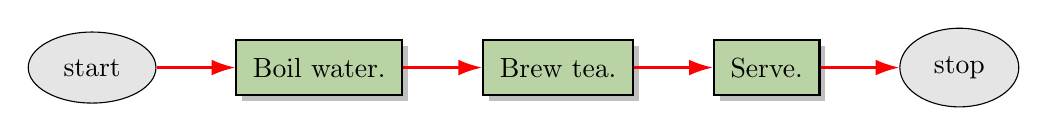
\begin{tikzpicture}[auto,
    -{Latex[length=3mm,width=2mm]},
    >=stealth
  ]
\node[st](start) {start};
\node[bb, right=of start](1) {Boil water.};
\node[bb, right= of 1](2) {Brew tea.};
\node[bb, right= of 2](3) {Serve.};
\node[st, right= of 3](stop) {stop};
\draw[kcedge] (start) to (1);
\draw[kcedge] (1) to (2);
\draw[kcedge] (2) to (3);
\draw[kcedge] (3) to (stop);
  \end{tikzpicture}
}
\end{center}

\end{frame}
% frame end %%%%%%%%%%%%%%%%%%%%%%%%

% frame begin %%%%%%%%%%%%%%%%%%%%%%%%
\begin{frame}[fragile]{Problem Decomposition}
{Making tea}
\begin{center}
\resizebox{\textwidth}{!}{
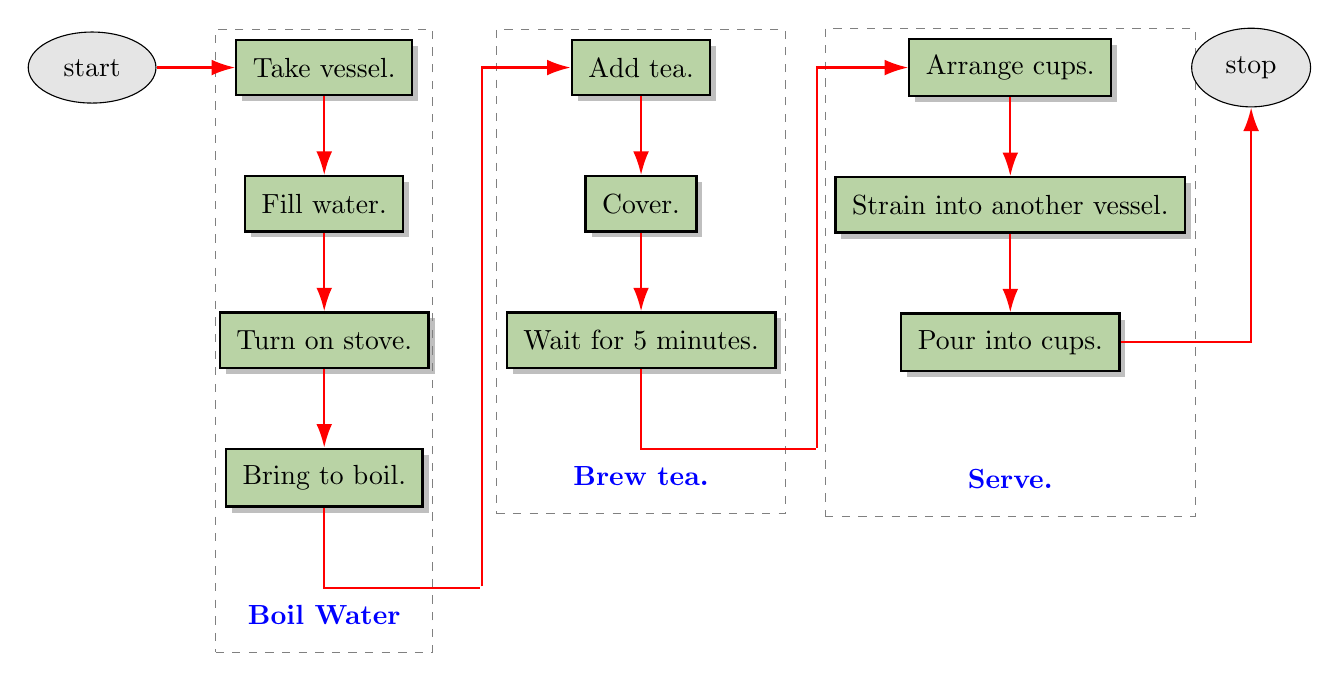
\begin{tikzpicture}[auto,
    -{Latex[length=3mm,width=2mm]},
    >=stealth
  ]
\node[st](start) {start};
\node[bb, right=of start](1_1) {Take vessel.};
\node[bb, below=of 1_1](1_2) {Fill water.};
\node[bb, below= of 1_2](1_3) {Turn on stove.};
\node[bb, below=of 1_3](1_4) {Bring to boil.};

\node[inv, below=of 1_4](l1) {\textbf{\color{Blue}Boil Water}};
\node[rectangle, draw=Gray, dashed, fill=none, fit=(1_1) (1_4) (l1)](1) {};

\draw[kcedge] (start) -- (1_1);
\draw[kcedge] (1_1) -- (1_2);
\draw[kcedge] (1_2) -- (1_3);
\draw[kcedge] (1_3) -- (1_4);

\node[bb, right=2 cm of 1_1](2_1) {Add tea.};
\node[bb, below=of 2_1](2_2) {Cover.};
\node[bb, below=of 2_2](2_3) {Wait for 5 minutes.};

\node[inv, below=of 2_3](l2) {\textbf{\color{Blue}Brew tea.}};
\node[rectangle, draw=Gray, dashed, fill=none, fit=(2_1) (2_3) (l2)](2) {};

\node[jn, below=of 1_4, xshift=2cm] (j1) {};
\draw[-, Red, thick] (1_4) |- (j1);
\draw[kcedge] (j1) |- (2_1);

\draw[kcedge] (2_1) -- (2_2);
\draw[kcedge] (2_2) -- (2_3);

\node[bb, right= 2.5 cm of 2_1](3_1) {Arrange cups.};
\node[bb, below= of 3_1](3_2) {Strain into another vessel.};
\node[bb, below= of 3_2](3_3) {Pour into cups.};
\node[inv, below=of 3_3](l3) {\textbf{\color{Blue}Serve.}};
\node[rectangle, draw=Gray, dashed, fill=none, fit=(3_1) (3_2) (l3)](3) {};

\node[jn, below right=of 2_3, xshift=-0.5cm] (j2) {};

\draw[-, Red, thick] (2_3) |- (j2);
\draw[kcedge] (j2) |- (3_1);
\draw[kcedge] (3_1) -- (3_2);
\draw[kcedge] (3_2) -- (3_3);

\node[st, right=of 3_1](stop) {stop};

\draw[kcedge] (3_3) -| (stop);
  \end{tikzpicture}
}
\end{center}

\end{frame}
% frame end %%%%%%%%%%%%%%%%%%%%%%%%

% frame begin %%%%%%%%%%%%%%%%%%%%%%%%
\begin{frame}[fragile]{Problem Decomposition}
{Advantages}

\begin{enumerate}
\item Allows step by step solution.
\item Reduces complexity by only retaining important details
\item Enables \emph{division-of-labour} and \emph{specialisation}.
\item
\begin{scriptsize}
\begin{itemize}
\item \textbf{Division of labour.} Ensuring that all \emph{team members/system components} are share the load equally.
\item \textbf{Specialisation.} \emph{Team members/system components} good at something get responsibilities aligned to their capability, and thereby get a chance to become better in their work.
\end{itemize}
\end{scriptsize}
\item Improves plan revision.
\item Improves \emph{modularity} (to be discussed in a later session).
\end{enumerate}
\end{frame}
% frame end %%%%%%%%%%%%%%%%%%%%%%%%

\end{document}
